\newpage
\chapter{Научни изчисления}
\label{chapter01}

Още в зората на съвременната изчислителна техника най-съществените пресмятания са били с научна насоченост и военно дело. Този факт не се е променил значително за последните десетилетия. Дори в наши дни най-сериозните изчислителни ресурси са насочени в областта на науката. Това дава основание да обърнем значително внимание на начините, по които можем да изпълняваме научни изчисления дори и върху изчислителни устройства, чието основно предназначение не е с научна цел. 

\section{Последователно програмиране}

При последователното програмиране\index{последователното програмиране} всяка изчислителна инструкция следва всички предходни. В зората на изчислителната техника пресмятанията са извършвани по този начин. Дори в наши дни значителна част от алгоритмите се изпълняват само последователно, тъй като входните данни за всяка инструкция зависят от изходните данни на предходните инструкции. Последователните алгоритми не подлежат на декомпозиране и поради тази причина са неприложими за паралелни пресмятания (Фиг. \ref{fig:pic0001}). 

\begin{figure}[h]
  \centering
  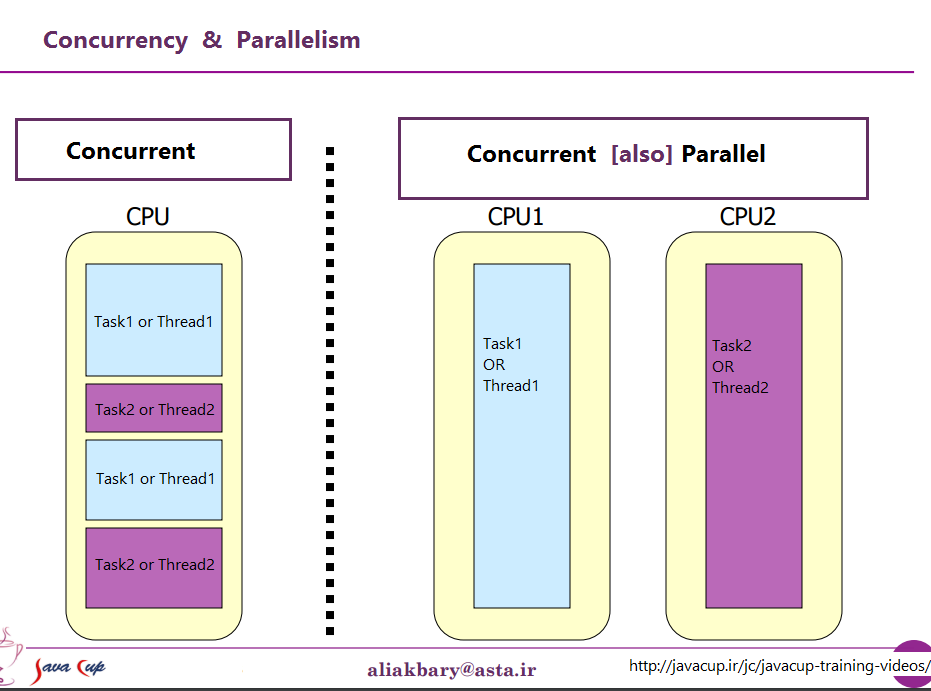
\includegraphics[width=1.0\linewidth]{pic0001}
  \caption{Сравнение между последователни пресмятания и паралелни пресмятания}
\label{fig:pic0001}
\end{figure}

\section{Паралелно програмиране}

При паралелното програмиране основно се говори за две разновидности - конкурентни пресмятания\index{конкурентни пресмятания} и паралелни пресмятания\index{паралелни пресмятания}. Конкурентните пресмятания са в среда, където група от задачи могат да се пресметнат едновременно без да има значение от реда на пресмятане. В същото време, паралелните пресмятания се отнасят за едновременно пресмятане на отделни задачи върху отделни процесори. В този контекст всички паралелни пресмятания са конкурентни пресмятания, но не и обратното (Фиг. \ref{fig:pic0002}). 

\begin{figure}[h]
  \centering
  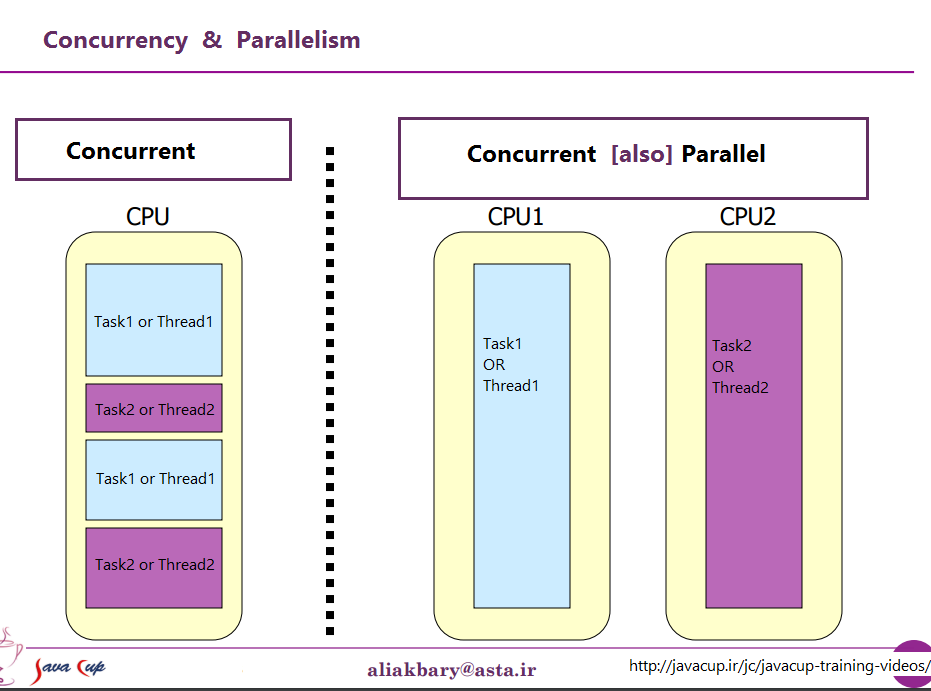
\includegraphics[width=1.0\linewidth]{pic0002}
  \caption{Сравнение между конкуретни пресмятания и паралелни пресмятания}
\label{fig:pic0002}
\end{figure}

\section{Супер компютри и грид изчисления}

Когато паралелните алгоритми се изпълняват на изчислителни машини с множество процесори и/или множество ядра на процесорите, този вид изчисления се определят като супер компютърни\index{супер компютърни изчисления} (supercomputing). Същественото при този вид пресмятания е, че се използва много бърза вътрешна шина (понякога оптична) и споделена оперативна памет. За разлика от супер компютрите\index{супер компютърни изчисления}, грид изчисленията\index{грид изчисленията} се осъществяват на множество машини свързани в обща мрежа, но работещи автономно без да споделят обща памет. При грид системите отделните изчислителни машини могат да са териториално отдалечени една от друга. Съществено е да се отбележи, че и при супер компютрите\index{супер компютърни изчисления} собственикът на системата има пълен контрол над нея. Това може малко да се различава за грид системите, ако към грида са включени компютри под чужд контрол. 

\section{Изчисления в разпределена среда}

Преходът от грид системите към системи за изчисления в разпределена среда\index{изчисления в разпределена среда} се състои в това, че изчислителните машини в разпределената среда са абсолютно автономни. Тези машини не споделят общи ресурси като процесор или оперативна памет. Много характерно е в разпределената среда контролът над изчислителните машини да не е от страната на организиращия изчисленията. Това води до два основни проблема - ненадеждна (често и твърде бавна) комуникация, липса на гаранция за коректност на пресмятанията (манипулации от страна на притежаващия изчислителните ресурси). Също така, при грид системите често се наблюдава хомогенност на изчислителните ресурси по отношение на хардуерни конфигурации и операционна система, докато в разпределената среда изчислителните машини са основно хетерогенни, което може да води до големи разлики в хардуера и операционните системи. 

\section{Дарена изчислителна мощност}

За решаването на някои по-мащабни научни проблеми изчислителната мощност и/или финансовите ресурси често са недостатъчни. В такива ситуации не малко научни институции прибягват до така наречените дарени изчислителни ресурси\index{дарени изчислителни ресурси} в разпределена среда\index{изчисления в разпределена среда}. Един от най-изчерпателните списъци с проекти от този вид може да бъде открит в уеб сайта Distributed Computing Info \cite{dcinfo}. Съществено е да се отбележи, че не всеки изчислителен проблем е подходящ за решаване в разпределена среда\index{изчисления в разпределена среда} с дарена изчислителна мощ. На първо място проблемът трябва да подлежи на декомпозиране, така че отделни части от него да се пресмятат едновременно. Второто важно нещо е да не е от съществено значение в кой момент от времето и в какъв ред ще бъдат получени пресметнатите резултати. И третото съществено нещо е да е наличен механизъм за проверка на достоверността от пресмятанията, тъй като изчисленията се извършват на машини с различна хардуерна конфигурация и различни операционни системи, а освен това са възможни манипулации от страна на хората притежаващи тези машини. Най-известният проект за дарена изчислителна мощ е SETI@home \cite{shuch} като неговата цел е да търси сигнали от космоса, които да са създадени от интелигентни форми на живот.

Когато изчисленията се извършват на мобилни устройства, то разпределената среда се превръща в мобилна среда за разпределени изчисления\index{мобилна среда за разпределени изчисления}. В останалата част от това учебно помагало ще бъде представено точно изграждането на система за извършване на разпределени изчисления върху мобилни устройства. 
